\documentclass[11pt]{article}
\usepackage{multicol}
% \usepackage{fullpage}
\usepackage{url}
\usepackage{graphicx}
\usepackage{natbib}
\usepackage{amsmath}
\usepackage{paralist}
\usepackage[small]{titlesec}
\begin{document}
\title      {\textbf{COMP6026: Assignment 2}}
\author	    {Thomas Smith\\taes1g09@ecs.soton.ac.uk}
\date       {\today}
\maketitle
% \begin{multicols}{2}
\section{Introduction}
% 1.5 pages
% o   Introduction: You need not spend more than 1.5 pages describing the original paper.
% ?         briefly describe the paper/experiment
% ?         What you evolved including
% ?         How you represented individuals
% ?         What fitness function did you define
% ?         What kind of GA you used
% ?         Steady state/ generational?  Tournament selection/ fitness proportionate (roulette wheel)?
% ?         What kind of crossover (if any) you used.
% ?         All parameters (enough detail so a reader could re-implement the GA)

%basic introduction
\citet*{orig} show that environmental conditions need not be externally imposed in order to promote the evolution of cooperative traits. They present a model which permits suitable conditions to arise via individual selection, and show that even in environments that initially select for selfish behaviour, a niche construction process can allow for cooperative behaviours to be ultimately successful. This paper reimplements the algorithm provided by \citet{orig}, and exends the model to show not only that the process is accelerated by the introduction of mutation to the model, but also that a side-effect of the niche construction process then favours selecting against individuals that are able to mutate, resulting in a more stable niche.




\section{Reimplementation}
%description of original paper
In \citet{orig}, an algorithm is presented which demonstartes that under the right circumstances, individuals can select for environments that promote cooperation


\begin{align} \label{eq:desire}
  r_i &= \frac{n_iG_iC_i}{\sum\limits_{j}(n_jG_jC_j)}R
\end{align}

\begin{align} \label{eq:shares}
  n_i(t+1) &= n_i(t) + \frac{r_i}{C_i} - Kn_i(t)
\end{align}

\begin{compactenum}
\item\textbf{Initialisation:} Initialise the migrant pool with $N$ individuals.
\item\textbf{Group formation (aggregation):} Assign individuals in the migrant pool
to groups, as described in the main text below.
\item\textbf{Reproduction:} Perform reproduction within groups for $t$ time-steps, as
described in the text above.
\item\textbf{Migrant pool formation (dispersal):} Return the progeny of each group
to the migrant pool.
\item\textbf{Maintaining the global carrying capacity:} Rescale the migrant pool
back to size $N$, retaining the proportion of individuals with each genotype.
\item\textbf{Iteration:} Repeat from step 2 onwards for a number of generations, $T$.
\end{compactenum}

\subsection{Representation}
For an efficient and quick algorithm, correct representation is important
First we did this
then we did this
Allowed quick computation, hooray

\subsection{Parameters}
We used the parameters as in the original paper, plus these

\begin{table}[!ht]
  \centering
  \begin{tabular}{r|c|ccr|c}
  Behaviour parameters	& Cooperative	& Selfish	&  & \multicolumn{1}{c}{} & \\ \cline{1-3}
  Growth rate, $G_i$			& 0.018			& 0.02		&  & Global parameters	& Value\\ \cline{5-6}
  Consumption rate, $C_i$		& 0.1			& 0.2		&  & Population size, $N$	& 4000\\
  \multicolumn{1}{r}{} & \multicolumn{1}{c}{} & \multicolumn{1}{c}{} &  & Generations, $T$ & 120 \\
  Size parameters		& Large			& Small		&  & Reproductions, $t$~ 		& 4\\ \cline{1-3}
  Group size, $S_i$			& 40			& 4			&  & Death rate, $K$ & 0.1\\
  Resource influx, $R_i$		& 50			& 4			&  & \multicolumn{1}{c}{} & \\
  \end{tabular}
  \caption{Parameters from \cite{orig}, used throughout the reimplementation.}
  \label{table:param}
\end{table}

\subsection{Results}
~1 page
% o   Reimplementated Results (~1 page)
% ?         The reimplemented figures (side by side with the originals)
% ?         Discussion of what the results show/don't show, what worked/didn't work, what you learned
\begin{figure}[!ht]
  \centering
  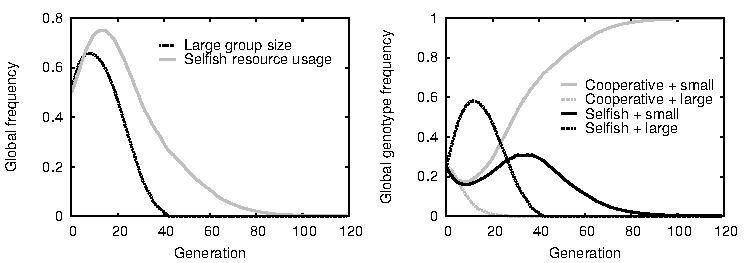
\includegraphics{equalplot.pdf}
  \caption{My plot.}
  \label{Figure:plot}
\end{figure}

\begin{figure}[!ht]
  \centering
  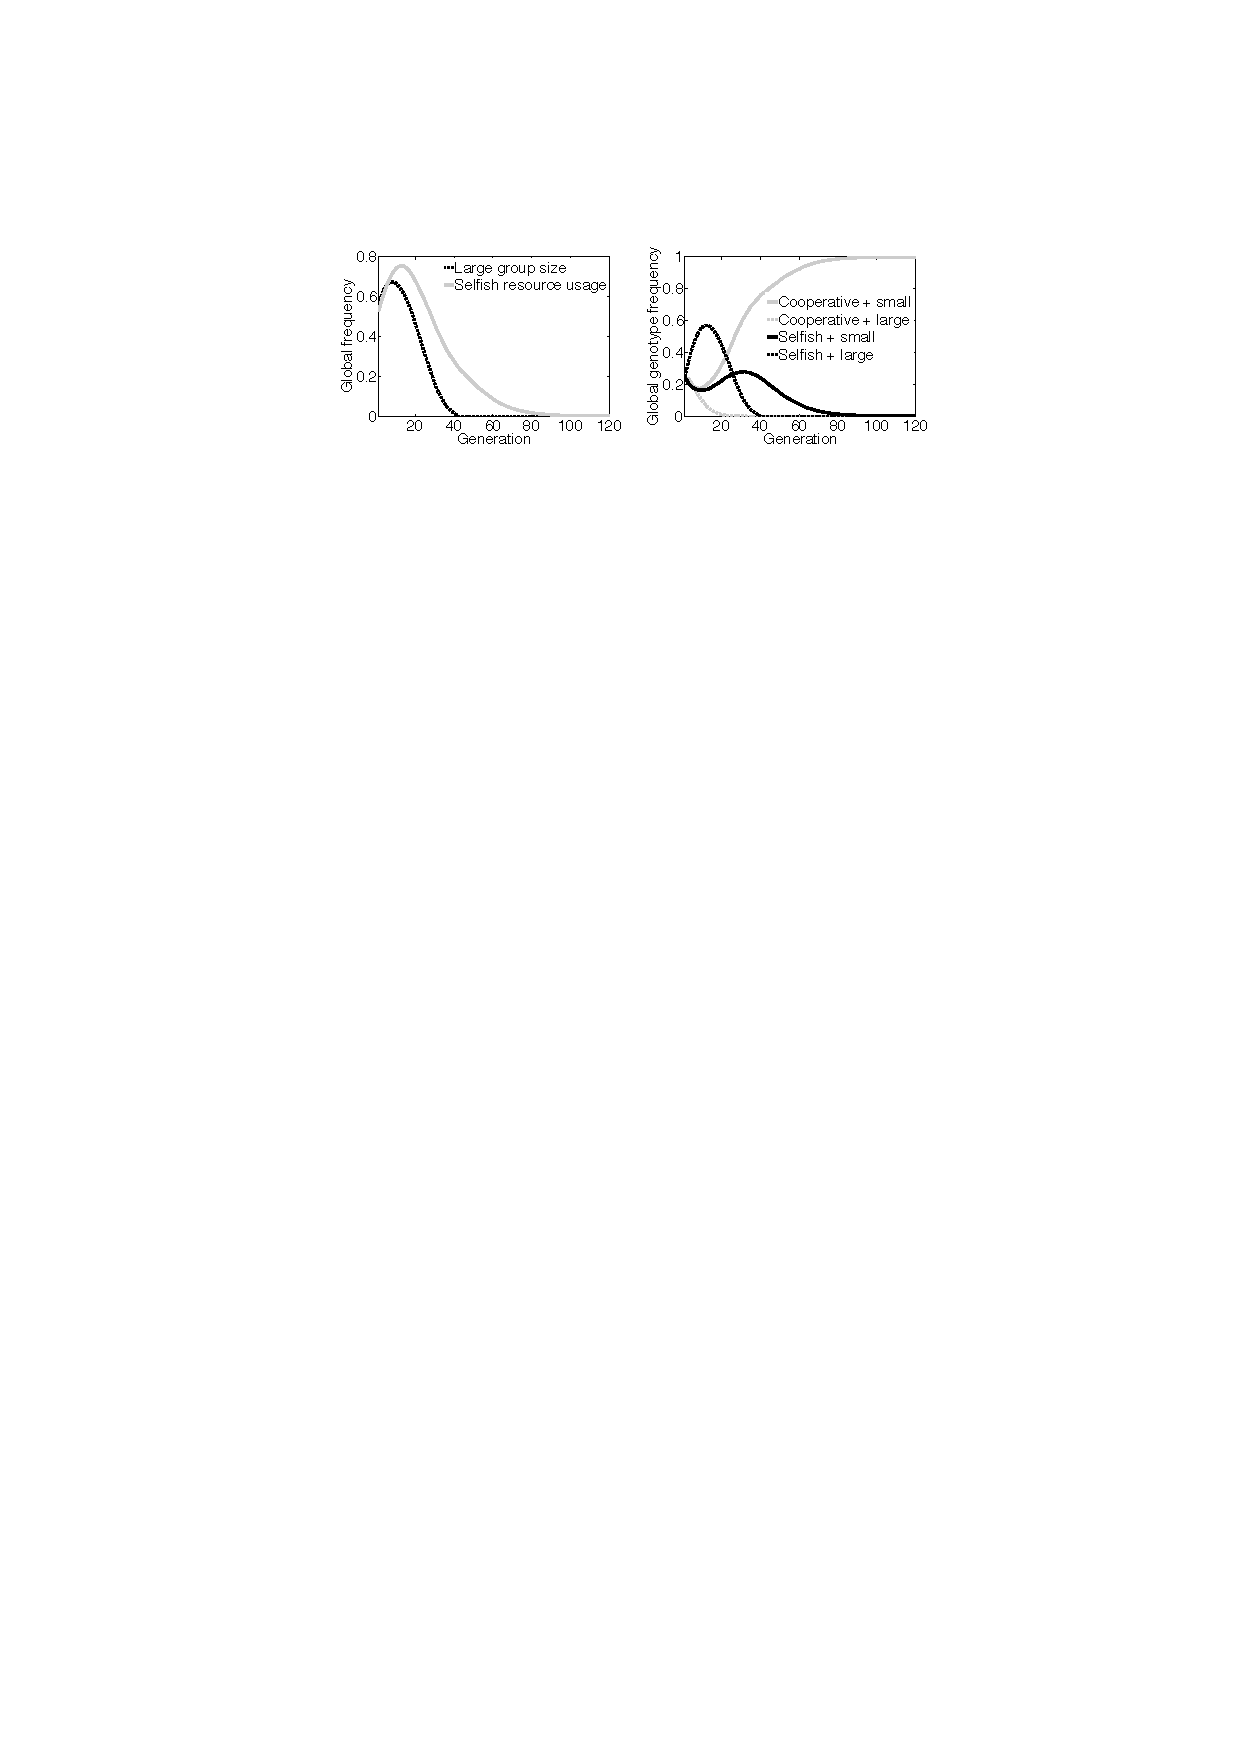
\includegraphics[scale=1.25]{original.pdf}
  \caption{original plot.}
  \label{Figure:original}
\end{figure}

\section{Extension}
~1 page
% o   Describe your extension  (another page)
% ?        What is your research question/hypothesis?
% ?         e.g., 'compare x with y' or 'add x and see what difference it makes compared to not(x)'.
% ?         Describe methods
% ?         Any advancements you made
% ?         Support the value of asking that question (using literature)
% ?         What do you expect to happen (what might happen)?
% ?         Why do you think that?

%choice of extionstion
a numenbt or extensiotns of the original paper exist
\citet{thesis} recommends altering the numebr of generations before breeding, or restiriction miigrations
thise papers have done these things

In the original paper, once a specific genotype has fixed, it is impossible for any other genotype to invade. Specifically, in order for any genotype to fix, all other genypes must be extinct.
What happens if we add mutatoin?
Are the results from the original paper robust in the face of new condidiotns
Several scenarios to consider:
 mutation only on size: predicatble results: once the selfish allele has died out, large + cooperative individuals that arise via mutation of the dominant small + cooperative genotype are able to flourish, and outcompete the other genotypes until they reach relative fixation (absolute fixation does not occur due to the occasional mutation of small + cooperative individuals).
 Mutation only on behaviour, and mutation on size and behaviour: i think leads to large + selfish near-fixation.
 Allowing individuals to select for the ability to mutate

\subsection{Representation}
Once again, individuals are represented by genotype as populations of identical clones. As there are three distinct alleles,there are now eight separate populations

\citet{optimal} notes that `optimal per-locus mutation rates depend mainly on $1/L$ (the reciprocal of the genotype length)'. In this model, the length of each individual's genotype is only 3, and a mutation rate of $1/3$ is high enough to cause no significant solution to arise. %I don't like the end of the sentence
However, the original reasoning behind the heuristic leads to a more effective value for mutation within the model. The use of a mutation rate of $1/L$ is intended to result in an average of one change to one gene in the individual per reproduction - in the model presented [TODO]% blah TODO
on the order of one change in one group per cycle of reproduction, and so a value of $1/num\_groups$ is more appropriate. Though the actual number of groups fluctuates based on prevailing group size preference, 550 groups may be taken as a reasonable approximation\footnote{~using the parameters in table~\ref{table:param} with equal distribution of genotypes: $\frac{2000}{40} + \frac{2000}{4} = 550$}. A mutation rate $M$ of $\frac{1}{550} \approx 0.002$ is therefore used throughout the rest of the paper.
\subsection{Results}
~1.5 pages
% o   Results of extension (another 1.5 page)

\section{Conclusion}
~1 page
% o  What do you conclude from that -- significance of the extension results/critique/evaluation (final page)

\bibliographystyle{plainnat}
\bibliography{EvoComp}{}
% \section*{References}
% \begin{thebibliography}{9}

% \bibitem{orig} 
% Powers, S., Penn, A., Watson, A.: Individual Selection for Cooperative Group Formation. Advances in Artificial Life: Proceedings of the Ninth European Conference on Artificial Life (ECAL 2007) (2007) 585--594

% \end{thebibliography}

\appendix
\section{Source}
% Appendix: source code of what you implemented (include the source of everything you implemented as part of the pdf)
% You may also upload a zip of all source code (if this includes any code you did not implement -- it must be clearly declared in a README file, and at the front of the report)

% \end{multicols}
\end{document}


What to include in your assign 2 report
See separate marks scheme for marking details.
o   Introduction: You need not spend more than 1.5 pages describing the original paper.
?         briefly describe the paper/experiment
?         What you evolved including
?         How you represented individuals
?         What fitness function did you define
? What kind of GA you used
?         Steady state/ generational?  Tournament selection/ fitness proportionate (roulette wheel)?
?         What kind of crossover (if any) you used.
?         All parameters (enough detail so a reader could re-implement the GA)
o   Reimplementated Results (~1 page)
?         The reimplemented figures (side by side with the originals)
?         Discussion of what the results show/don't show, what worked/didn't work, what you learned
o   Describe your extension  (another page)
?        What is your research question/hypothesis?
?         e.g., 'compare x with y' or 'add x and see what difference it makes compared to not(x)'.
?         Describe methods
Any advancements you made
?         Support the value of asking that question (using literature)
What do you expect to happen (what might happen)?
Why do you think that?
o   Results of extension (another 1.5 page)
o  What do you conclude from that -- significance of the extension results/critique/evaluation (final page)
Appendix: source code of what you implemented (include the source of everything you implemented as part of the pdf)
You may also upload a zip of all source code (if this includes any code you did not implement -- it must be clearly declared in a README file, and at the front of the report)
 

 particular aggregation and dispersal metapopulation structure that we have modelled. 